\documentclass[sigconf]{acmart}

\usepackage{graphicx}
\usepackage{hyperref}
\usepackage{todonotes}

\usepackage{endfloat}
\renewcommand{\efloatseparator}{\mbox{}} % no new page between figures

\usepackage{booktabs} % For formal tables

\settopmatter{printacmref=false} % Removes citation information below abstract
\renewcommand\footnotetextcopyrightpermission[1]{} % removes footnote with conference information in first column
\pagestyle{plain} % removes running headers

\newcommand{\TODO}[1]{\todo[inline]{#1}}

\begin{document}
\title{Big Data Analytics in Finance Industry}


\author{Gagan Arora}
\orcid{HID301}
\affiliation{%
  \institution{Indiana University}
  \date{October 2017}
}
\email{gkarora@iu.edu}


% The default list of authors is too long for headers}
\renewcommand{\shortauthors}{B. Trovato et al.}


\begin{abstract}
Discusses the importance of Big data, data classification, cross industry comparison and analytic and its impact on finance industry and how customer satisfaction can be improved to achieve competitive advantage 
\end{abstract}

\keywords{Big data,finance, data classification,HID301, data type, big data impact, cross-industry comparison, banking, customer personalization, pattern recognition, multi document summarization, structured and unstructured data}


\maketitle

\section{Introduction: Discuss importance, how dominating }

By its nature of the business, the finance industry is always driven and dominated by data. The existence of Big data in the finance industry has exposed the big opportunity of growth and value extraction but at the same time imposed the various new challenges, which demand new skill set. \cite{Ref3} suggests that finance experts believe there is a huge potential in terms of value extraction from the financial big data. They also believe that finance industry can benefit more than any other industry.  Historically, data was always there in some format either non-digital or digital. However, with digitalization, this data has fallen into the prevalence of high volume of information, which we call as Big Data. Dominant drivers for the actuality of big data in the finance industry are mainly customer call logs, social media, news feed, regulatory data etc. Call logs, news feed and etc. fall into the category of unstructured data which is identified as an area where we can extract vast amount of business value. We will discuss the various types of data, which is being generated at a phenomenal rate and what business value can be extracted out of big data. We will also discuss what all challenges this big data imposes on the finance industry. \cite{Ref1} talks about the effectiveness of extracting value out of big data in the finance industry and utilizing it to improve business operation. 

\section{Market impact: Pace at which market is adding data}

\cite{Ref2}  talks about the three V of big data in finance industry: volume, velocity and variety. We will also discuss the fourth V aspect of it in a later section, which is a vulnerability. Fig 1 \cite{Ref3} clearly depicts the amount of financial data pouring in the daily basis. TechNavio’s forecast (Technavio 2016) predicts data will grow at a CAGR [compound annual growth rate] of 61 percent over the period of 2017-2021. According to the IDC financial insight 2016, every second there is around 10,000-payment card transaction and this number is expected to double by the end of this decade. The Capgemini/RBS Global payments study for 2012 suggests there was about 260 billion transactions in 2012 and is expected to grow between 15 and 22 percent for developing countries. Main drivers contributing to the big data in the finance industry are Data growth, increasing scrutiny from regulators, digitalization of financial products, changing the business model and increased customer insight platforms such as customer service.  Fig 2 [\cite{Ref2}] shows 76 percent of banks say the business driver for embracing big data is to enhance customer engagement, retention, and loyalty and 71 percent of banks say that to increase their revenue, they need to better understand customers and big data will help them to do so. 

\section{Competition/problem: How peer industry adding data and their initiative  }

Thinking about the data strategy, the financial industry has taken the business-driven approach to a big data. According to the IBM report, all financial organizations are not keeping the same pace as peer industry is keeping. Today because of increased competition, customers always expect more personalized banking service and at the same time, there is increased regulatory surveillance which in result creates big pressure on finance industry to better utilize the value of Big data. To achieve better-personalized experience, many banks have started the initiative to utilize the information gained from the vast ocean of data to offer better-personalized products and gain competitive advantage.  Despite the fact that financial industry is data-driven, there is a gap in the amount of initiative financial industry has taken to extract the value out of big financial data.  Technavio 2016 report has shown only 26 percent of financial organizations has focused on understanding the principal notation of Big data and most of those 26 percent are still struggling to define the clear roadmap. This clearly concludes that finance industry lag behind their cross-industry peers in using more varied data types. A good example to support this fact is that there are very less research and domain knowledge in extracting value out of retail bank call logs. 

\section{Why big data in Finance and its impact on the customer personalization and their satisfaction}

Big data technologies not only help in extracting the effective business value but analysis of unstructured data in conjunction with a wide variety of data set also helps in extracting commercial value. Big data in finance industry does not necessarily decode to valuable or actionable information. The real benefit lies in developing the technologies, which can be used to extract business and commercial value.  \cite{Ref4}  talks about what all advantage we can extract from the big data in the finance industry. Few examples are: Detection of false rumors that try to manipulate the finance market, Assessment of exposure to a reputational risk connected to consulting service offered by banks to their customer and Discover topic trends, detect events, or support the portfolio optimization or asset allocation.  Big data based pattern recognition can also help in enhanced fraud detection systems and prevention capability systems. Other benefits of utilizing big data include building a machine learning based algorithm to achieve higher performance and accuracy in the trading algorithm and Enhanced market trading analysis. There has been proven research \cite{Ref7} which states more data increases accuracy and precision of simulations which is the backbone of financial modeling based analytics. This research \cite{Ref7} states Modern modeling techniques are data hungry 

\section{Big data classification in finance industry: structured un-structured and semi-structured }

Financial service system has a varied variety of data pools that are held by various stakeholders. At a high level of abstraction, we can classify them into three major categories: Structured data, Unstructured data, and Semi-structured data. With the emergence of too much data supply, there has been operational intelligence initiative such as firms like SPLUNK which uses data mining approaches to fetch valuable information out of any type of log. There have been studies \cite{Ref6} which shows utilizing structured data for analyzing event logs. Another advantage of structured data is that it makes the concept of Data Virtualization easy as data can easily be virtualized if we have structured data, which in turn make easy to extract patterns. Extracting patterns from the customer banking activities gives banks competitive advantage as they can make better personalized financial products for customers. 

\subsection{Structured data}

This reflects the data which has a higher degree of an organization such as a relational database where information/data is easily searchable and we can easily apply standard algorithm to extract patterns out of it. Examples of such data set include Trading applications, Enterprise finance resource planner, Retail banking systems, Credit history database systems and other financial applications that use legacy application systems. Structured data always has a big advantage of being easily entered, stored, queried and analyzed. Most of the personal banking financial statements are stored in a structured way. Structured dataset combined with the distributed systems can be leveraged to achieve Structured big data set on which we can run optimized SQL queries to retrieve patterns. \cite{Ref5}  discusses various SQL based ways to specify information quality in data which can be used to filter out the noise. 

\subsection{Unstructured data}

With the emergence of social media, blogging and mobile usage there has been a phenomenal amount of data which we can classify as unstructured data. Example of unstructured data includes Daily stock feeds, Company announcements, Finance news, Articles, Blogs, Customer feedback/reviews and etc. There have been researches such as multi-document summarization and machine learning algorithms to utilize the unstructured data to extract value.  There is a big advantage with the unstructured data that it is a platform, programing language, technology compatible ie. Two or more machines which different platform can interact with each other using unstructured data. This means financial big unstructured data can be stored on distributed systems and pattern recognition application can be used to extract value.   There are also other ways such as transforming unstructured data to structured and then fetching intelligence out of it since structured data is akin to machine language. 

\subsection{Semi-structured data}

As the name suggests this data type includes the aspect of both structured as well as an unstructured data type. Examples of semi-structured data includes: Financial products markup language[FpML], Financial Information eXchange[FIX], Interactive Financial eXchange(IFX), Open Financial eXchange(FEDI) , Market data definition language (MDDL) and etc. \cite{Ref1} suggests nowadays semi-structured data dominates the data in finance industry which contributes to around 80-85 percent of finance data

\section{Various Challenges utilizing Big data value in finance industry }

There are multiple challenges and constraints in extracting value out of big financial data. The biggest challenge is old IT culture and infrastructure. The Much financial organization still uses old IT infrastructure which is not compatible with the big data application thus fail to take advantage of big data. Other challenges include lack of skill set and data privacy and security. With the emergence of digitalization, customer data is saved persistently because of which there has been continued concern regarding the customer privacy. Regulatory bodies guidelines on customer data are always ill-defined because of which is there is always a concern regarding the use of customer data.  

\section{Requirements Solution and Conclusion }

In this section, we will discuss various technical requirements needed to achieve value extraction from the big data in the finance industry. There are various technical requirements such as Data Acquisition, Data Quality, Data Extraction, Data Integration, Decision support. In order to fulfill requirements, a hybrid approach combining computer science, algorithms, statistics, data mining, machine learning and pattern recognition study needs to be adopted. To explore the advantage of big data there have been initiatives like data virtualization, multi-document summarization, pattern recognition from LOGS and many start-ups have been emerged.  All big companies such as Microsoft, Google, IBM and Amazon are investing heavily in this field to leverage business and commercial value out of it. There has been changed in the industry pattern where financial industry is resorting big data to strategize their business. According to \cite{Ref3}  with a very rapid pace, the financial industry is utilizing big data advantage in investment analysis, econometrics, risk assessment, fraud detection, trading, customer interaction analysis and behavior modeling. If we look at the Big promise the Big data holds in the finance industry, progress in this field is still in nascent stage and we expect more growth in upcoming years.  

\begin{figure}[p!]
    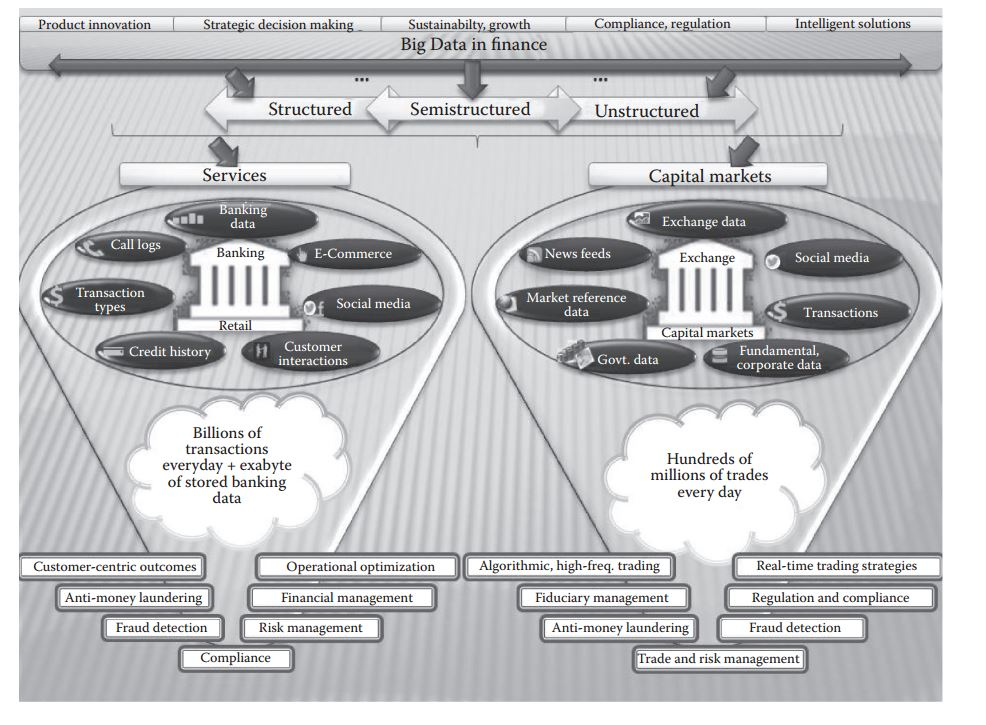
\includegraphics{images/dataTypes.JPG}
    \caption{Figure 1}
    \label{fig:figure1}
\end{figure}

\begin{figure}[p!]
    \includegraphics{images/bankingBigData.JPG}
    \caption{Figure 2}
    \label{fig:figure2}
\end{figure}

\bibliographystyle{ACM-Reference-Format}
\bibliography{report} 

\section{Bibtex Issues}
\todo[inline]{Warning--empty chapter and pages in editor00}
\todo[inline]{(There was 1 warning)}
\section{Issues}

\DONE{Example of done item: Once you fix an item, change TODO to DONE}

\subsection{Formatting}

    \TODO{Incorrect number of keywords and i523 not included in the keywords}

\subsection{Writing Errors}

    \TODO{A few punctuation errors}

\subsection{Structural Issues}
    \TODO{Abstract is too short and lacks an introductory sentence}

\subsection{Details about the Figures and Tables}

    \TODO{In case you copied a figure from another paper you need to ask for copyright permission. In case of a class paper, you must include a reference to the original in the caption}
    \TODO{The figure's caption must include a meaningful description of the figure, along with citation of the reference from which the image is copied}
    \TODO{Do use {\em label} and {\em ref} to automatically create figure numbers. Refer to them in the text properly}
    \TODO{Remove any figure that is not referred to explicitly in the text (As shown in Figure ..)}   
    \TODO{Figures should be reasonably sized and often you just need to
  add columnwidth} e.g. \begin{verbatim}/includegraphics[width=\columnwidth]{images/myimage.pdf}\end{verbatim}

re
\end{document}
